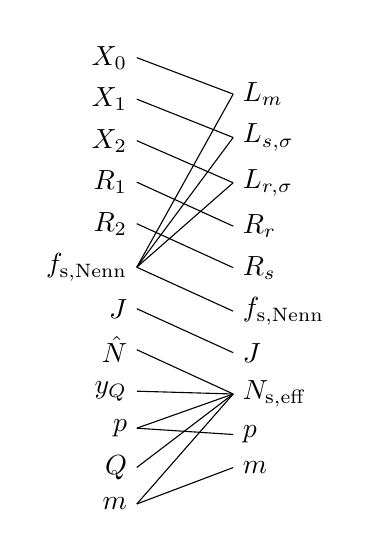
\begin{tikzpicture}[node distance=.5cm]
    % Linke Seite
    \begin{scope}[]
    	    \matrix[column 1/.style={anchor=base east}]{
             \node[] (X0) {$X_0$}; \\
             \node[] (X1) {$X_1$}; \\
             \node[] (X2) {$X_2$}; \\
             \node[] (R1) {$R_1$}; \\
             \node[] (R2) {$R_2$}; \\
             \node[] (fsNennl) {$f_{\mathrm{s,Nenn}}$};\\
             \node[] (Jl) {$J$};\\
             \node[] (N) {$\hat N$};\\
             \node[] (yQ) {$y_Q$};\\
             \node[] (pl) {$p$};\\
             \node[] (Q) {$Q$};\\
             \node[] (ml) {$m$};\\
        };
    \end{scope}
    % Rechte Seite
    \begin{scope}[xshift=2.5cm]
    	    \matrix[column 1/.style={anchor=base west}]{
             \node[] (Lm) {$L_m$}; \\
             \node[] (Lssigma) {$L_{s,\sigma}$};\\
             \node[] (Lrsigma) {$L_{r,\sigma}$};\\
             \node[] (Rr) {$R_r$};\\
             \node[] (Rs) {$R_s$};\\
             \node[] (fsNenn) {$f_{\mathrm{s,Nenn}}$};\\
             \node[] (J) {$J$};\\
             \node[] (Neff) {$N_{\mathrm{s,eff}}$};\\
             \node[] (p) {$p$};\\
             \node[] (m) {$m$};\\
        };
    \end{scope}
    \draw (Lm.west) edge (X0.east)
                    edge (fsNennl.east);

    \draw (Lssigma.west) edge (X1.east)
                    edge (fsNennl.east);

    \draw (Lrsigma.west) edge (X2.east)
                    edge (fsNennl.east);

    \draw (Neff.west) edge (N.east)
                      edge (pl.east)
                      edge (Q.east)
                      edge (ml.east)
                      edge (yQ.east);

    \draw (Rr.west) edge (R1.east);

    \draw (Rs.west) edge (R2.east);

    \draw (fsNenn.west) edge (fsNennl.east);

    \draw (p.west) edge (pl.east);

    \draw (m.west) edge (ml.east);

    \draw (J.west) edge (Jl.east);
\end{tikzpicture}

%             \node[] (XN) {$X_N$}; \\
%             \node[below=of XN] (XD) {$X_D$}; \\
%             \node[below=of XD] (XD') {$X_D'$}; \\
%             \node[below=of XD'] (XD'') {$X_D''$}; \\
%             \node[below=of XD''] (XQ) {$X_Q$}; \\
%             \node[below=of XQ] (XQ'') {$X_Q''$}; \\
%             \node[below=of XQ''] (XS) {$X_S$}; \\
%             \node[below=of XS] (fsN) {$f_{s,N}$}; \\
%             \node[below=of fsN] (Rs) {$R_s$}; \\
%             \node[below=of Rs] (TD0') {$T_{D0}'$}; \\
%             \node[below=of TD0'] (TD'') {$T_D''$}; \\
%             \node[below=of TD''] (TQ'') {$T_Q''$}; \\